\subsection{Screenshots}\label{l:screenshots}

\setlength\fboxsep{2pt}
\setlength\fboxrule{0.5pt}

\begin{center}
\fbox{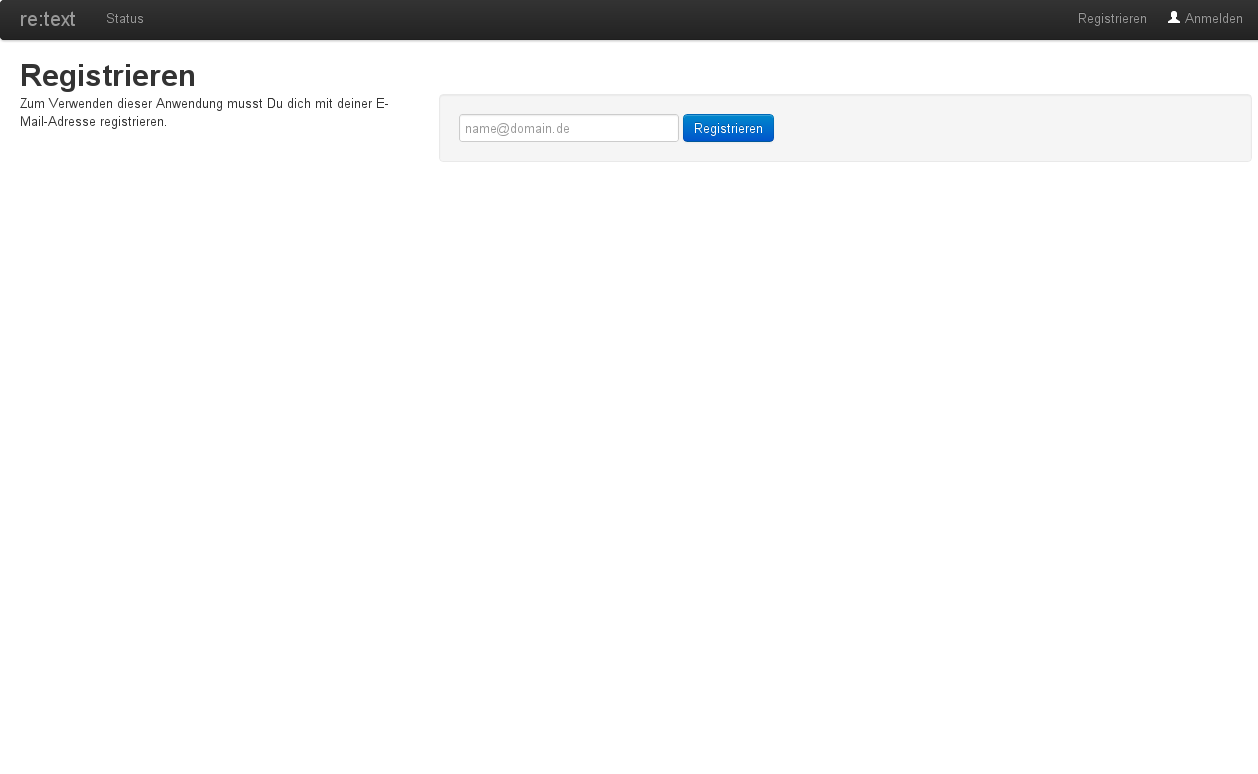
\includegraphics[width=0.95\textwidth]{media/screenshots/app/register.png}}
\captionof{screenshot}{Registrierung für neue Benutzer}
\end{center}

\begin{center}
\fbox{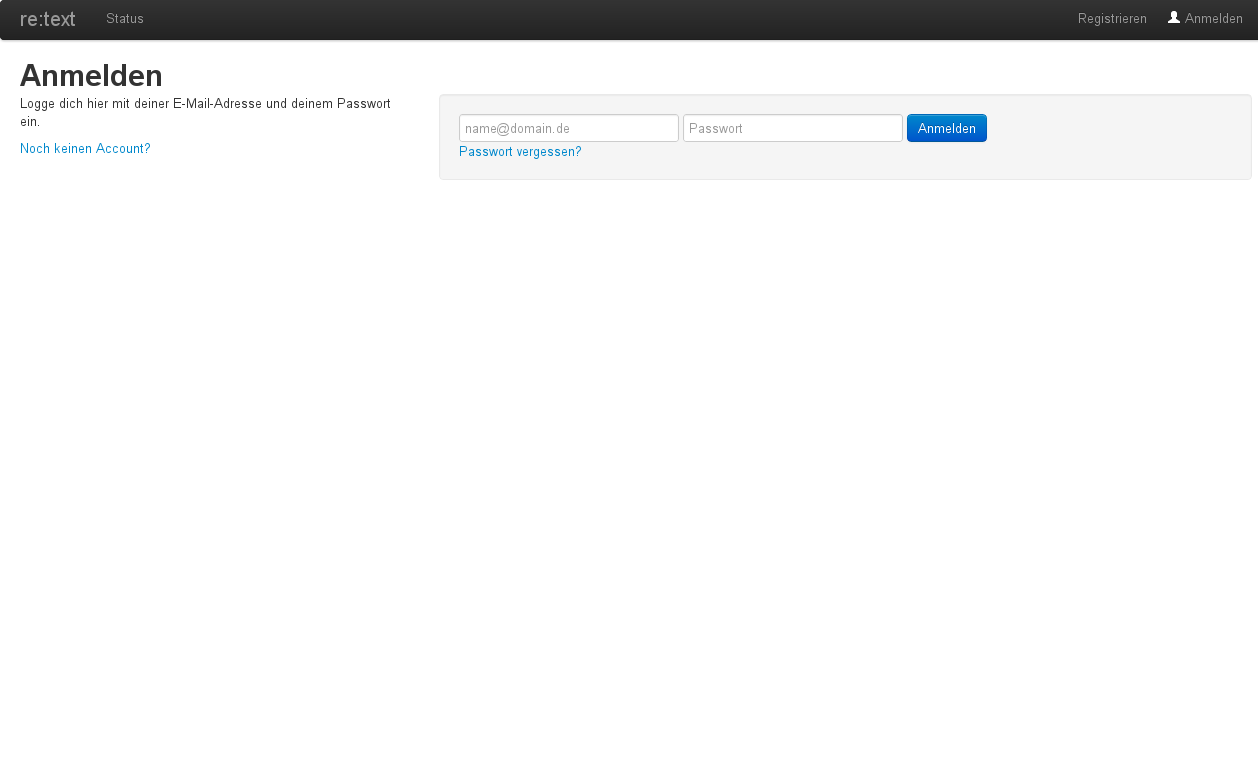
\includegraphics[width=0.95\textwidth]{media/screenshots/app/login.png}}
\captionof{screenshot}{Login}
\end{center}

\begin{center}
\fbox{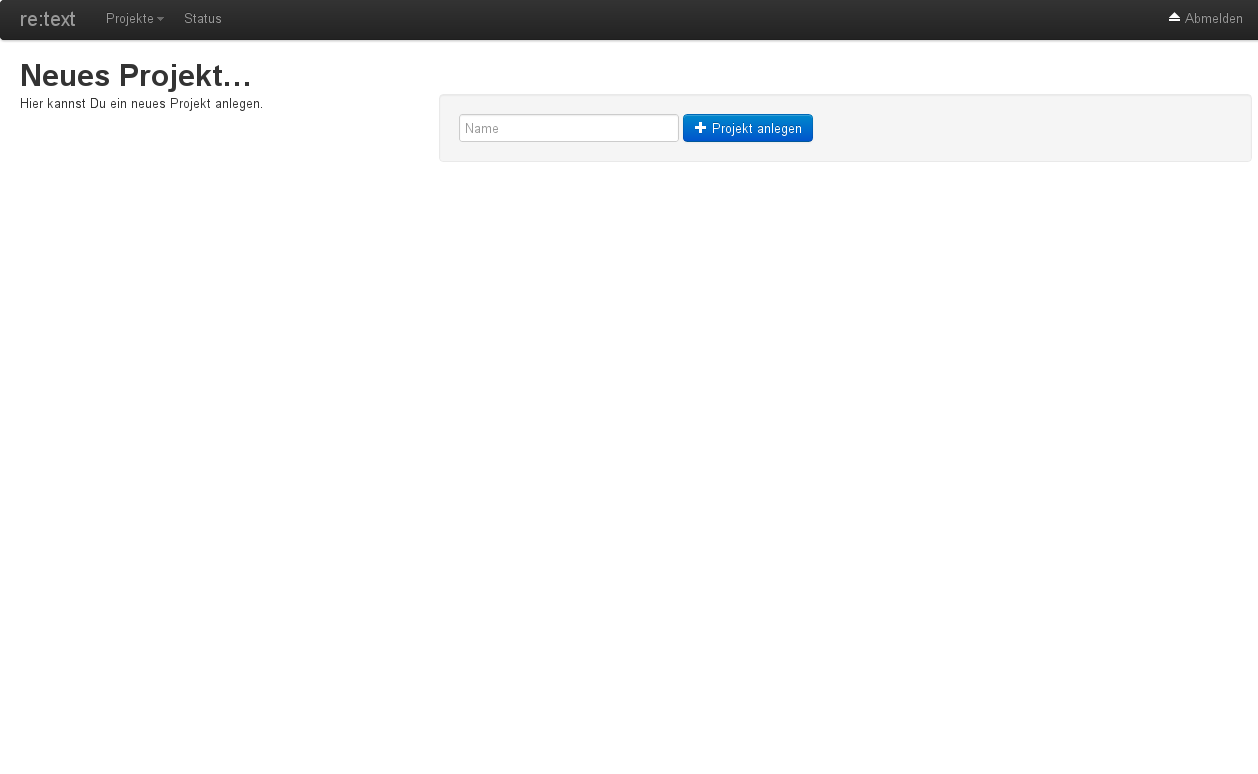
\includegraphics[width=0.95\textwidth]{media/screenshots/app/newproject.png}}
\captionof{screenshot}{Projekt anlegen}
\end{center}

\begin{center}
\fbox{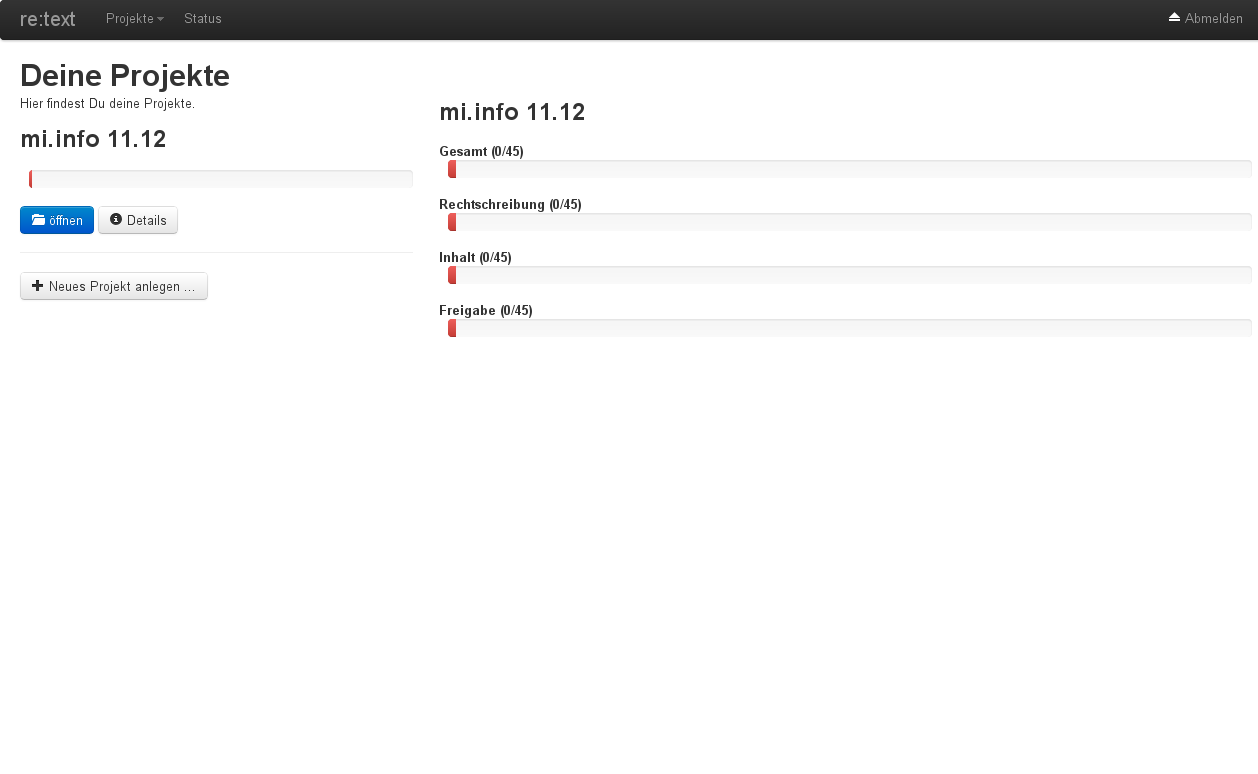
\includegraphics[width=0.95\textwidth]{media/screenshots/app/showproject.png}}
\captionof{screenshot}{Projekt anzeigen, mit Darstellung des Projekt-Fortschritts}
\end{center}

\begin{center}
\fbox{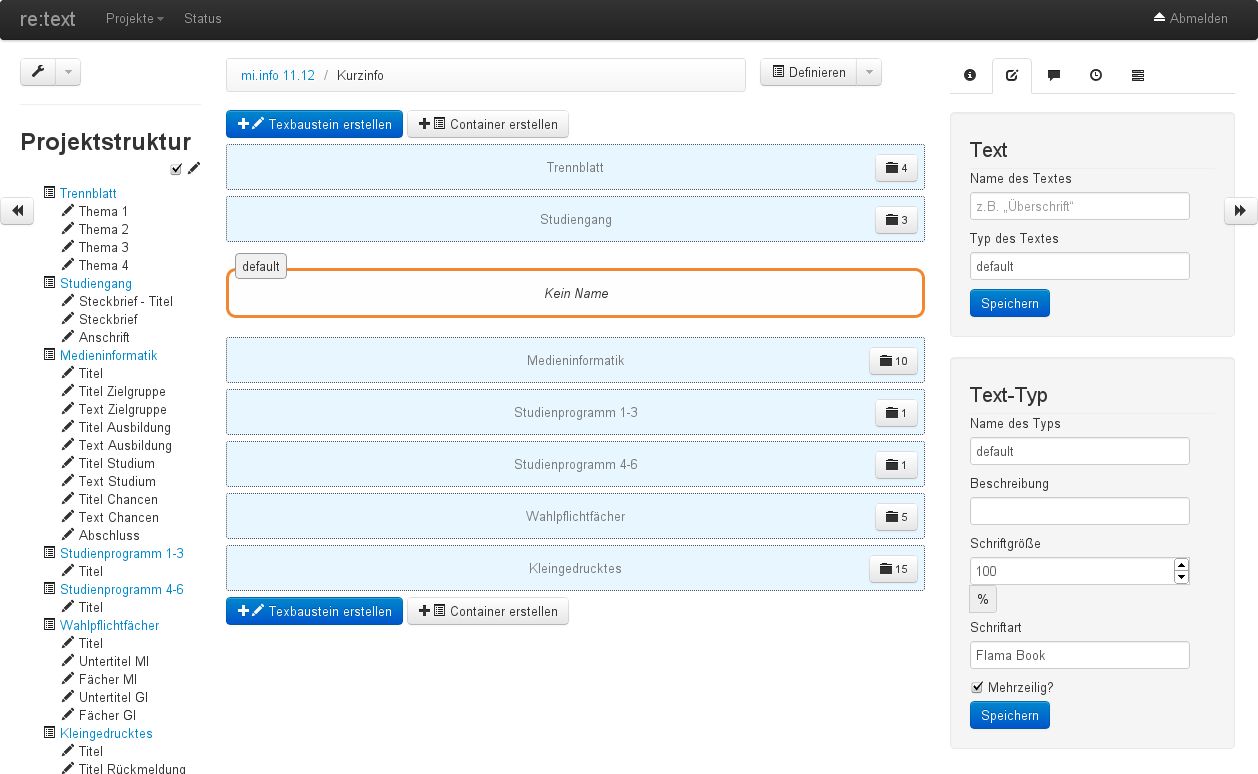
\includegraphics[width=0.95\textwidth]{media/screenshots/app/structure.png}}
\captionof{screenshot}[Produktstruktur definieren]{Produktstruktur definieren, vgl. \ref{l:gui-definition}~·~S.\pageref{l:gui-definition}}
\end{center}

\begin{center}
\fbox{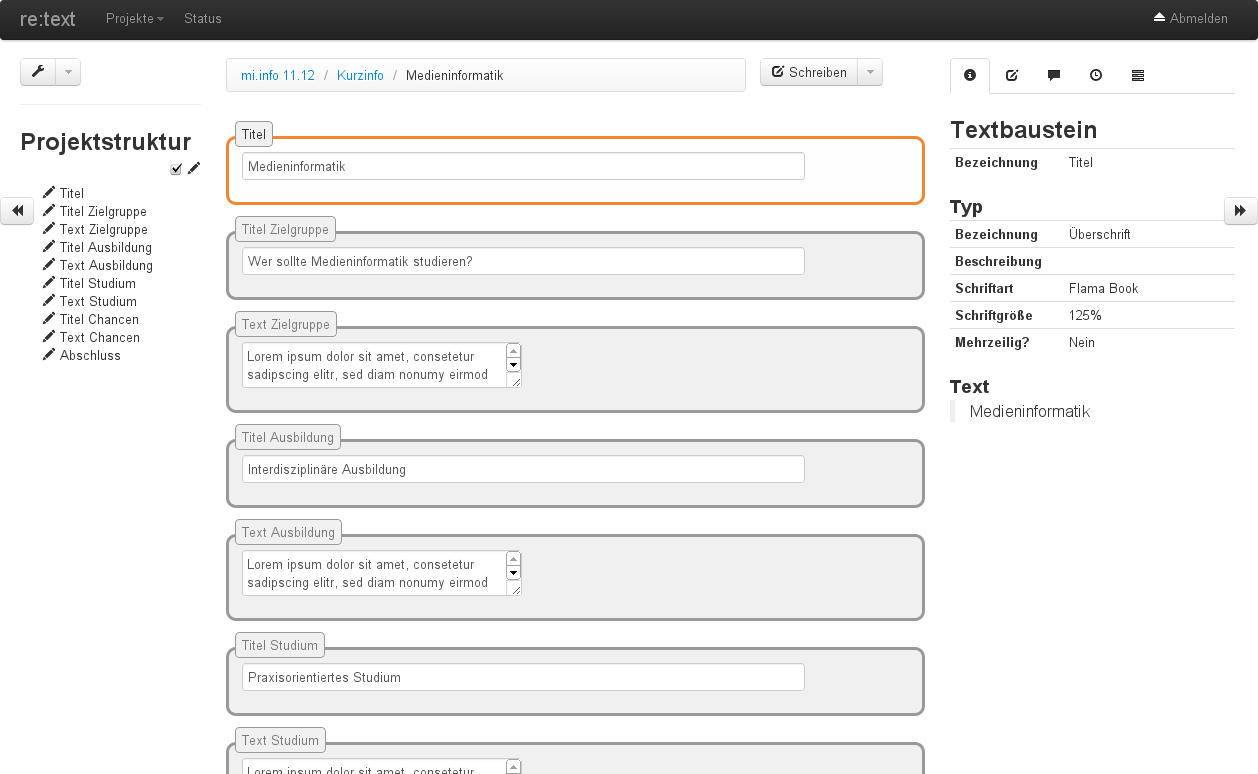
\includegraphics[width=0.95\textwidth]{media/screenshots/app/write.png}}
\captionof{screenshot}[Texte erstellen]{Texte erstellen, vgl. \ref{l:gui-texten}~·~S.\pageref{l:gui-texten}}
\end{center}

\begin{center}
\fbox{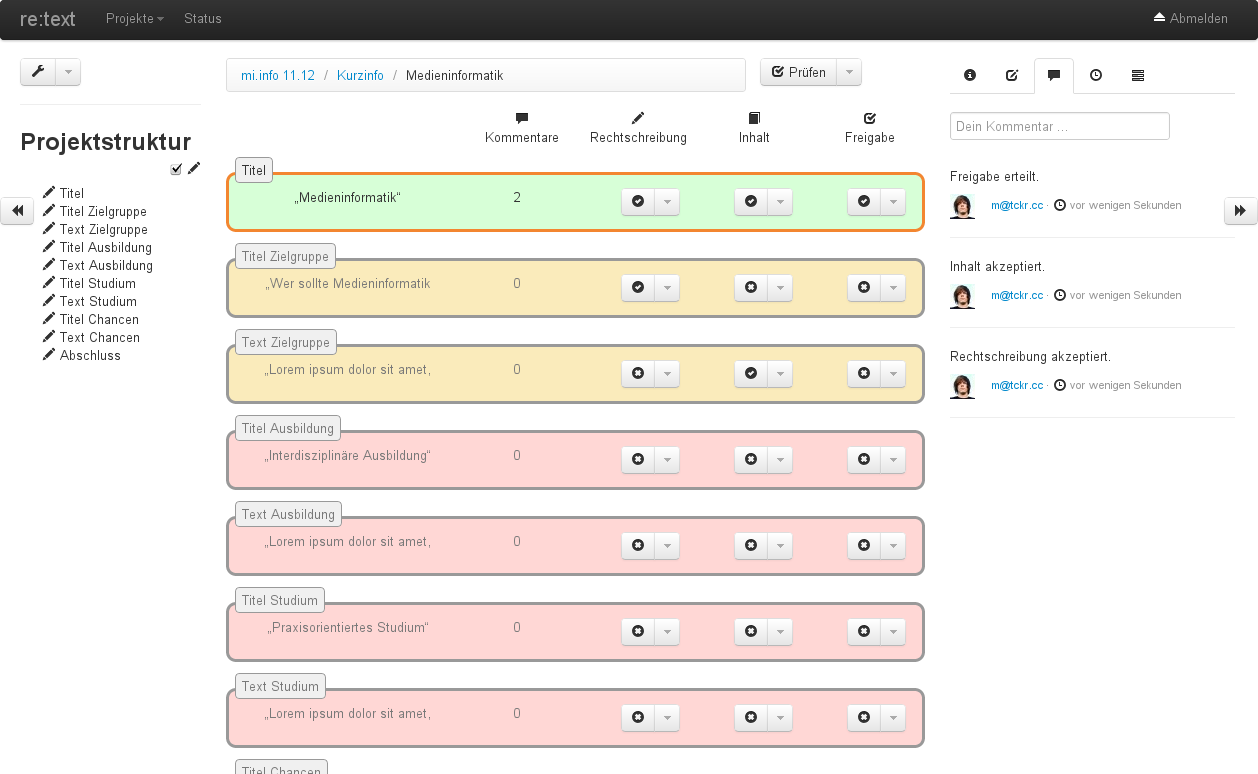
\includegraphics[width=0.95\textwidth]{media/screenshots/app/check.png}}
\captionof{screenshot}[Qualitätssicherung]{Qualitätssicherung, vgl. \ref{l:gui-qs}~·~S.\pageref{l:gui-qs}}
\end{center}

\begin{center}
\fbox{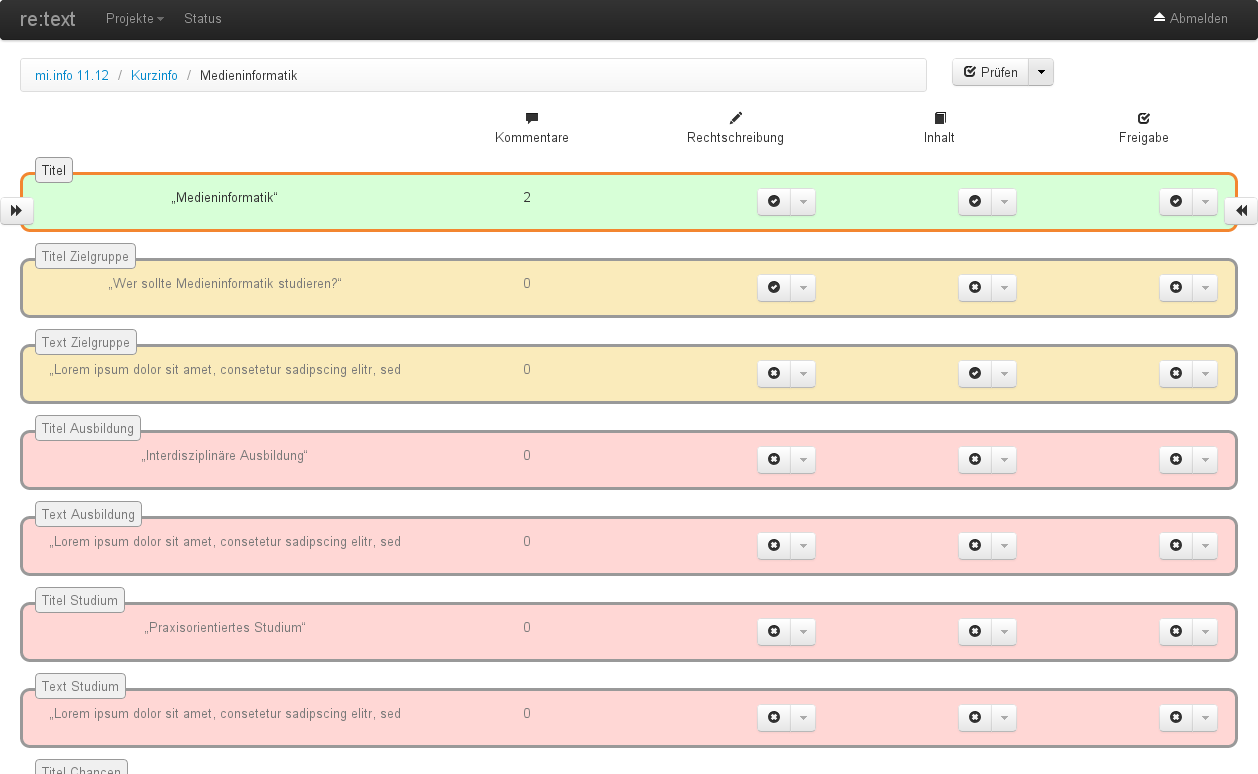
\includegraphics[width=0.95\textwidth]{media/screenshots/app/fullscreen.png}}
\captionof{screenshot}[Darstellung im Vollbild-Modus mit ausgeblendeten Seitenleisten]{Darstellung im Vollbild-Modus mit ausgeblendeten Seitenleisten, vgl. \ref{l:gui-aufbau}~·~S.\pageref{l:gui-aufbau}}
\end{center}

\pagebreak